\chapter{Contenidos educativos con el robot mBot}\label{cap:aplicationEducativa}
En este capítulo proporcionaremos una propuesta educativa  basada en ejercicios prácticos, cuyo objetivo global es el aprendizaje de robótica y pensamiento computacional, y de sus principios y conceptos básicos. \\
Estos ejercicios prácticos utilizan dos herramientas diferentes, cuyo orden temporal es fijo por lógica educativa: la primera herramienta, Scratch, la nativa del fabricante del robot mBot, es más sencilla al no ser un lenguaje de programación al uso. Una vez superada la primera fase de aprendizaje, será posible pasar a un lenguaje de programación de texto con sintaxis, compilación, ejecución por comando, etc, utilizando Python y la plataforma diseñada en este Trabajo Fin de Grado. 

\section{Enseñanza de robótica y programación con el robot mBot}\label{sec:enseñanzarobotica}
 Con el objetivo de enseñar pensamiento computacional y programación a jóvenes y de provocar un interés a corto y largo plazo en ello, la robótica es el encuadre perfecto. Utilizando una herramienta que contemplan como un juego, seremos capaces de guiarles en conceptos aparentemente complejos, programación, algoritmia, etc, de forma intuitiva y simple, sin entrar en compleja teoría que les haría perder la atención e interés. El robot elegido y las herramientas software utilizadas y previamente explicadas, componen un marco lo suficientemente simple para ser utilizado sin problemas y sin necesidad de conocimientos previos, proporcionando a la vez suficiente capacidad para las enseñanzas y objetivos perseguidos.
\subsection{Contexto}\label{subsec:contexto}
Los ejercicios de Scratch explicados a continuación no son el resultado de un diseño meramente teórico, sino que fueron puestas en práctica durante un curso completo, en el marco de unas clases extraordinarias de robótica, a alumnos y alumnas de Educación Primaria en el colegio Nuestra Señora de Rihondo, en Alcorcón (Madrid). Pudo comprobarse la acogida y la efectividad de los contenidos, en algunos casos adaptando la dificultad o añadiendo pasos a la primera versión del ejercicio si fuera necesario. \\
La plataforma Python original, PyBoKids\cite{JdeRobot}, requería de una instalación de JdeRobot y el simulador Gazebo, compleja, en Linux. Durante el curso escolar, se comprobó que esta era poco adaptable a un curso  completo de alumnos. Para este Trabajo Fin de Grado diseñamos por tanto, una versión de la plataforma que poder usar fácilmente en un contexto de clase colectiva. No es necesario instalar nada, aparte de Python, en los equipos (normalmente equipos de escuela, de prestaciones limitadas). De hecho, dado que el residente completo va grabado en el robot y no es necesario cambiar el programa grabado cuando se quiera usar una práctica diferente, no es necesario instalar siquiera Arduino. Sólo será necesaria la instalación de Python y el archivo \textit{.py} correspondiente a la biblioteca de PyBoKids-2.0 \\
Las prácticas descritas para la segunda parte son una transcripción de algunas prácticas de Scratch (las relativas a aplicaciones), adaptadas a los periféricos disponibles en PyBoKids-2.0 y con las limitaciones físicas que conllevan tener el robot conectado por cable al PC (para mantener la comunicación entre Python y el canal Serial). 


\subsection{Metodología}\label{subsec:metodología}
Las metodologías de cualquier tipo de programación son perfectamente utilizables en robótica y en el trabajo con jóvenes. La más intuitiva de ellas, de hecho la que ellos mismos utilizan de una forma natural (aunque no completamente ordenada), es \textit{Agile}\footnote{Filosofía de Desarrollo web basada en iteraciones}. Sin embargo, a los estudiantes no les explicaremos explícitamente que estamos usando este método, sino que diseñaremos los ejercicios con el fin de que deba usarse, y les guiaremos durante la ejecución con este método. 
\begin{figure}[h]
	\centering
	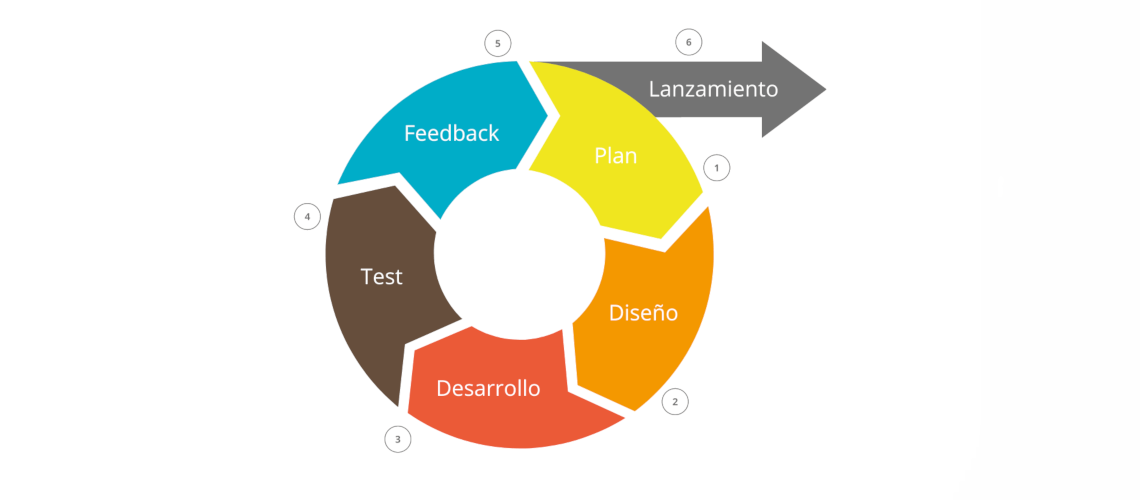
\includegraphics[scale=0.3]{agile.png}
	\label{img:agile}
	\caption{Esquema de una iteración Agile}
\end{figure}
Aunque las etapas de una iteración Agile clásica son cinco (\textit{Plan, Diseño, Desarrollo, Test y Feedback}), al ser Scratch y las prácticas un entorno muy sencillo, haremos con éstas un Agile simplificado, fusionando las fases de Plan y Diseño, que con los alumnos serán trabajo común. Las fases de Test y Feedback no las fusionaremos propiamente, sino que las haremos a la vez y poniendo las ideas en común: probando el ejercicio en el robot y comprobando si el comportamiento es el deseado. \\
Durante las clases, la metodología será de trabajo en común para el planteamiento del ejercicio, e individual (o por parejas dependiendo del ratio de robot por persona) para el desarrollo y el test.

\section{Programación robótica con Scratch}\label{sec:scratch}
Las prácticas de esta etapa están pensadas con unos objetivos docentes individuales, y otros globales con respecto al curso completo de ejercicios. Además, no podemos perder de vista que, para los estudiantes, las clases de robótica deben ser \textit{entretenidas}; dado que no son curriculares es importante mantener su atención creando ejercicios dinámicos y diferentes cada vez, además de con contenido educativo. 
\subsection{Makeblock}\label{subsec:makeblock}
Antes de pasar a describir las prácticas diseñadas, hablaremos de la plataforma nativa para la programación del robot mBot: \textit{mBlock}, del fabricante Makeblock\cite{makeblock}, y cómo lo utilizaremos en las clases. \\
Como hemos adelantado en el Capítulo \ref{cap:infra}, donde explicamos su instalación y uso básico, el fabricante pone a disposición un aplicativo, disponible para PC y dispositivo móvil (o tablet), para programar el robot mBot (y todos sus modelos de robot) con el lenguaje Scratch de una forma muy intuitiva. Este software es muy útil para la programación con jóvenes sin experiencia: requiere solamente de la instalación del software, y tiene integrados la forma de conectar con el robot y de grabar el código de un programa en la placa.\\
\begin{figure}[h]
	\centering
	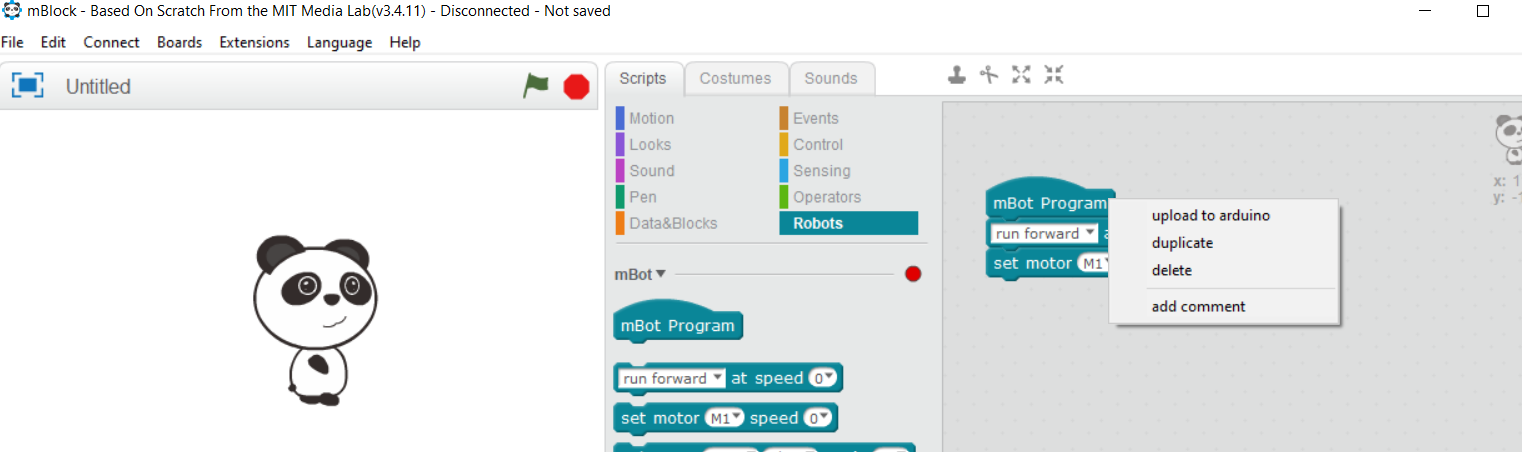
\includegraphics[scale=0.5]{mblock_ejemplo.png}
	\label{img:pantallamblock}
	\caption{Aplicación mBlock: pantalla inicial}
\end{figure}

En nuestro caso, lo utilizaremos durante las clases en la primera parte del curso, orientada a la solución de los ejercicios con Scratch. 
Para ello, el propio alumno/a hará el proceso inicial de actualización de firmware, sólo necesario una vez, y de conexión mBlock-Robot (esta, sin embargo, será necesaria cada vez, puede verse en el propio programa si el robot está conectado o no). Este procedimiento está explicado en la sección \ref{list:conexionMblock}. \\
El proceso de solución de un ejercicio utilizando Scratch y mBlock, siguiendo los objetivos Agile marcados, es el siguiente:
\begin{enumerate}
	\item Discusión sobre el problema planteado, toma de requerimientos común.
	\item Diseño de un esquema de solución con soporte visual (pizarra), y separación del problema completo en pequeños ejercicios unitarios (\textit{bottom-up})
	\item Programación en Scratch del primer problema unitario
	\item Grabación en el robot del programa (ver en la figura \ref{img:uploadArduino}) diseñado. Para grabar el programa, será necesario que el robot esté conectado por USB al PC, encendido y establecida la conexión entre PC y mBlock
	\item Prueba de la solución unitaria. Para ello, podemos desconectar el robot, ya que el programa está grabado en la placa (no hay ningún programa ejecutando en el PC que requiera mantener la conexión). Es notable el hecho de que, nada más subir el programa a la placa, comenzará a funcionar. Para poder ejecutar el programa ''desde cero en limpio'', podremos apagar el robot una vez hayamos grabado el programa, y volverlo a encender donde o cuándo queramos probar la solución. La placa Arduino ejecutará el programa que tenga grabado desde cero cada vez que se encienda, hasta que otro programa sea grabado.
	\item Continuación hasta la solución completa.
\end{enumerate}
\subsection{Prácticas con actuadores} \label{subsec:practicasactuadores}
 Como se ha explicado anteriormente, el propósito de un actuador es ejecutar la orden que recibe de la placa. Es, por tanto, muy visual y conveniente para introducir el curso de robótica, pues da pie a equivocarse y aprender de los errores de forma mucho más intuitiva que con otros componentes.
 
\begin{description}

\item [Carreras]\label{ej:carreras}
Obviamente, lo más visual del robot mBot son los motores. También es lo más intuitivo y esperable de un robot en general: que se mueve por sí mismo. Es uno de los componentes más sencillos de programar, ya que Scratch ofrece un desplegable con los posibles valores que aceptan los motores del mBot. Además, tiene métodos directamente para avanzar, retroceder y girar, muy cómodos para el primer contacto con el robot y válidos para este ejercicio en concreto. \\
En vez de simplemente \textit{mover} el robot, el ejercicio se pensó como una carrera entre los robot de todos los alumnos, para despertar su interés y hacerlo más entretenido; sin una utilidad práctica, o un juego, los alumnos perdían interés rápidamente o, incluso, no lo tenían desde el principio. \\
\textbf{Ejercicio Extra} Otro punto que se pudo comprobar con la experiencia empírica es que era mejor hacer varias versiones de un mismo ejercicio, aunque la dificultad fuera la misma, con objetivos distintos. Los alumnos no pierden la atención y aprenden que una misma solución, con pequeñas variaciones, vale para distintas situaciones. Además, así queda cubierta la situación de que los alumnos vayan a distintas velocidades y unos terminen el ejercicio base mientras otros no.\\
Otra versión de este ejercicio de carreras es hacerla con obstáculos fijos. Los alumnos tendrán que medir en tiempo la distancia entre obstáculos y jugar, con las velocidades y los giros. Quién mejor combinación encuentre, mejor tiempo hará en carrera.\\
Con este ejercicio, con sus diferentes versiones de obstáculos y de distancias, introducimos el concepto de actuador, explicando en clase la definición, y también el concepto de robot (primer concepto que se comentará y al que volveremos repetidamente durante el curso para revisar la definición que den los estudiantes). También el concepto de ``programación secuencial temporal'', ya que para evitar los obstáculos deberán programar Scratch para avanzar durante \textit{x} tiempo, después girar, volver a avanzar, etc.
\begin{figure}[h]
	\centering
	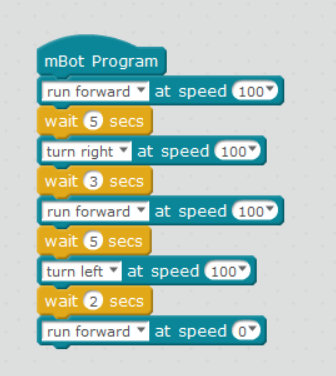
\includegraphics[scale=1]{carreras.png}
	\label{img:carreras}
	\caption{Ejemplo de solución al ejercicio ``Carreras''}
\end{figure}
\begin{figure}[H]
	\centering
	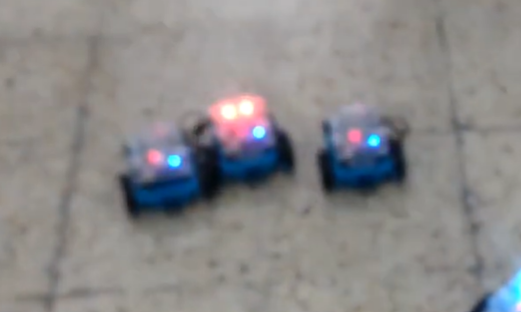
\includegraphics[scale=0.6]{carrerasrobot.png}
	\label{img:carrerasrobot}
	\caption{Uso en clase del ejercicio de carreras}
\end{figure}
\item [Cumpleaños feliz]\label{ej:cumple}
Otro actuador sencillo de usar es el zumbador integrado en la placa. Es algo más complicado, pues las notas musicales no son las más conocidas y, sobre todo en los alumnos más jóvenes, no están acostumbrados a una escala musical. Sin embargo, se puede comprobar que no tardan mucho en entender el sistema de escalas; se les ayudará dándoles la tabla de equivalencias entre las notas americanas y europeas.
\begin{table}[H]\centering
	\begin{tabular}{||ccccccc||}
		\hline
		Do & Re & Mi & Fa & Sol & La & Si \\[1.5pt]
		C & D & E & F & G & A & B \\
		\hline
	\end{tabular}
	\caption{Equivalencia entre notas}
\end{table}

Una vez entendida la diferencia de notas y comprobado cómo funciona el zumbador, les proponemos que el robot entone la canción de cumpleaños feliz - o cualquier otra 	que seguro conozcan-. No sólo sirve para el actuador, sino que introducimos el concepto de repetición (bucles). La idea principal es dejarles al principio que hagan el ejercicio todo seguido y después les ayudamos a entender que están repitiendo código: hay estrofas que se repiten. Ven la necesidad, pues, de meter esas estrofas dentro de un bucle de repetición de tantas veces como sea necesario.

\textbf{Ejercicio Extra}. Una vez han terminado la primera canción, es bueno invitarles a que intenten que el robot \textit{cante} otras melodías que conozcan y les apetezcan.

\item [S.O.S.]\label{ej:sos}
El siguiente actuador del pack del mBot son las luces LED de la placa, el rango de colores RGB permite que cada alumno pueda personalizar los colores como más les guste. El propio lenguaje Scratch permite el rango de cada color entre 0 y 255 (aunque en la práctica, no sean notables los cambios pequeños en esa escala).\\
La finalidad del ejercicio es que, con luces, el robot pida ayuda en lenguaje morse: tres pulsos cortos, tres pulsos largos, y tres pulsos cortos. \\
Como se ha comentado anteriormente, los alumnos son más proactivos cuando ven una utilidad mínimamente real a lo que se les pide, y conocen el lenguaje morse -o es muy sencillo de explicar- y la utilidad de pedir ayuda en un lenguaje universal.\\
En este ejercicio reforzamos las duraciones; el progreso temporal de las órdenes. Los puntos y rayas del morse los traducimos a esperas de menos y más tiempo, respectivamente. También reforzaremos el concepto de bucle, pues el mensaje podremos repetirlo con un bucle en vez de repitiendo todas las órdenes.  En las figuras \ref{img:SOS} y \ref{img:SOSrobot} puede verse un ejemplo de solución propuesta y su aplicación. Podemos ver el resultado real de hacer el ejercicio en clase en vídeo\footnote{\href{https://www.youtube.com/watch?v=k6QSnIkRVyo}{https://www.youtube.com/watch?v=k6QSnIkRVyo}}. \\
\begin{figure}[h]
	\centering
	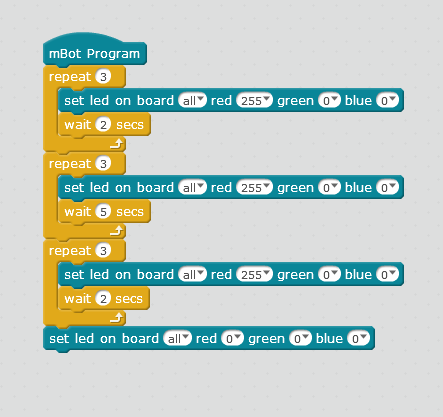
\includegraphics[scale=1]{SOS.png}	
	\caption{Ejemplo de solución para el mensaje S.O.S. en morse}
	\label{img:SOS}
\end{figure}
\begin{figure}[h]
	\centering
	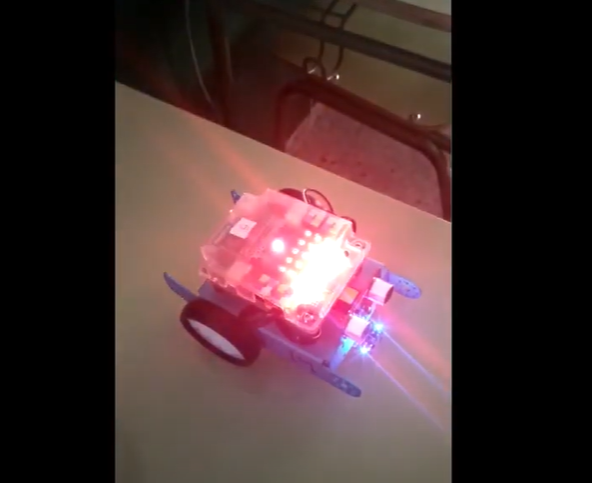
\includegraphics[scale=0.4]{SOSrobot.png}	
	\caption{Uso del ejercicio S.O.S en morse en clase}
	\label{img:SOSrobot}
\end{figure}
\textbf{Ejercicio Extra}. Una vez que han conseguido que el mensaje de socorro sea entendible, cambiamos el ejercicio a escribir en morse cualquier mensaje que se les ocurra (con la tabla de equivalencias del abecedario) y a mandar el mismo mensaje de socorro con luz y sonido a la vez.

\item[Camión]\label{ej:camion}
Como último ejercicio de actuadores, intentaremos juntarlos todos, a la vez que todavía no introducimos ningún sensor. Proponemos, pues, emular el comportamiento de un camión, algo a lo que están acostumbrados y que no se les habría ocurrido que era automatizable. Un camión, haga lo que haga, si da marcha atrás, pitará (con los zumbadores) y encenderá las luces naranjas. \\
Vamos metiendo, poco a poco, acciones simultáneas, para que tengan que preocuparse de más de un componente (de más de un bloque de Scratch). El objetivo es el aprendizaje de que, en robótica, un comportamiento aparentemente trivial es la suma de muchos comportamientos simultáneos y dependiente uno de otro.\\
Con este ejercicio, aprendemos el concepto, tan necesario en la programación de robótica, de \textit{concurrencia}. Cuándo, y sólo cuándo, el camión da marcha atrás, es cuando se encienden las luces y sirenas.
\begin{figure}[h]
	\centering
	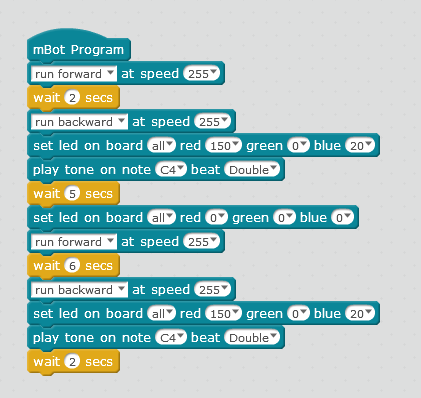
\includegraphics[scale=1.1]{camion.png}	
	\caption{Ejemplo de solución para el ejercicio del camión}
	\label{img:camion}
\end{figure}
\end{description}

\subsection{Prácticas con sensores} \label{subsec:practicassensores}
Los sensores recogen información del medio y la devuelven en forma numérica. Es misión del programador, pues, procesar el retorno y la interpretación de esa información de forma correcta, unívoca y cubriendo todos las posibilidades. \\
Esto requiere unas habilidades más avanzadas, además de los conceptos básicos de programación como bucles, condicionales, concurrencias, etc, que se han visto en los ejercicios anteriores de actuadores. Los alumnos deberán ser capaces de:
\begin{enumerate}
	\item Decidir qué información necesitan del entorno para el problema que se les presenta. Es decir, dividir el problema en pequeños trozos hasta llegar al más pequeño de ellos. Éste será del que tengan que abstraer el tipo de información que necesitan conocer para poder solucionarlo.
	\item Una vez conocida la información que necesitan, deberán elegir qué sensor es el que mejor les va a dar esa información. Al principio, será una cuestión trivial, pues sólo habrá una posibilidad, pero después introduciremos ejercicios que requieran de varias \textit{informaciones} distintas, por lo cual, de varios sensores.
	\item Tras obtener del sensor el valor de retorno numérico, es misión del alumno diseñar la respuesta de vuelta del robot, es decir, cómo deba comportarse dependiendo de esa respuesta. No será lo mismo si queremos acercar el robot a un muro lentamente para aparcar, que si debemos tener cuidado de que no choque o si debe perseguir a otro robot: el sensor es el mismo, y el valor de retorno también, pero el comportamiento no tiene por qué ser el mismo. 	
	\item Fijándose en la necesidad original, y en las repuestas que se reciben de cada sensor, deberán ser capaces de granular la sensibilidad del sensor, o del valor de control, para obtener un comportamiento lo más refinado y preciso posible (siempre teniendo en cuenta las limitaciones técnicas del mBot).
\end{enumerate}

Estas habilidades las iremos trabajando poco a poco, diseñando ejercicios que las introduzcan a la vez, pues son necesarias todas, pero con diferentes niveles de dificultad.\\
Como siempre, en cada ejercicio iremos guiando a los alumnos en la división del problema de forma \textit{bottom-up}; esta división de los problemas es una de las habilidades más importantes en programación, y una de las cosas sobre las que más haremos hincapié.

\begin{description}
	
\item [No chocar contra un muro]\label{ej:muro}
Uno de los actuadores más visibles, y por el que los alumnos siempre preguntan, es el sensor de proximidad (sensor de ultrasonidos). El bloque de Scratch para este sensor devuelve un valor numérico, la distancia a la que se encuentra del obstáculo que esté leyendo. Por tanto, para los alumnos es tan cómodo como trabajar con ``distancia x del sensor''. \\
Este ejercicio se diseñó con el mismo ánimo que el del camión (\ref{ej:camion}), siguiendo la idea de que programen cosas que conocen, que utilizan en su día a día, con el fin de que aprendan la idea que la robótica está incluida en nuestras vidas y cualquiera puede dedicarse a ello.\\
El objetivo es, por tanto, programar el sensor de proximidad de los coches, que cuando aparcan y se acercan al coche de delante (en este caso, a un muro), primero pita, si te acercas más pita más rápido y, al final, se para. Como es el primer sensor que utilizan, lo orientaremos en etapas. \\
Primero, necesitan aprender cómo se usan el sensor y el valor de retorno. Es decir, el bloque de Scratch que llama al sensor no sirve de nada sin añadirlo a algún otro bloque que utilice el valor que el sensor lee del entorno (por ejemplo, un bloque condicional). Este primer ejercicio lo haremos utilizando directamente el bloque de lectura del sensor; más adelante introduciremos el concepto de variable.\\
Después, tendrán que conseguir la parte difícil del ejercicio: que el robot se pare cuando se acerque al muro. Así comprobarán de forma real cómo funciona el sensor, además de ajustar la sensibilidad de ''cuánto de cerca'' debe estar el robot para considerar que está pegado al muro pero para qué dé tiempo a pararlo sin que se choque.\\
Una vez conseguida esta primera parte, que requiere de bloques condicionales, de concurrencia o de espera (no hay una sola forma correcta de hacerlo), solucionar el ejercicio completo es -relativamente- inmediato. El comportamiento deseado es que, cuando el robot se acerque un poco al muro, pite ligeramente (con el zumbador de la placa, que ya se ha utilizado antes; véase \ref{ej:cumple}); cuando se acerque algo más, pite más intensamente y, cuando esté muy cerca (la distancia que se haya decidido en la primera parte del ejercicio), parará para no chocar.
En las figuras, \ref{img:muro1} y \ref{img:muro2}, podemos ver ejemplos de la realización del ejercicio durante las clases; también pueden en vídeo\footnote{\href{https://www.youtube.com/watch?v=dMYWTzXvXlE}{https://www.youtube.com/watch?v=dMYWTzXvXlE}} \footnote{\href{https://www.youtube.com/shorts/HWSd4kJJ7kY}{https://www.youtube.com/shorts/HWSd4kJJ7kY}}. \\

\begin{figure}[h]
	\centering
	
	\begin{subfigure}
		[Un ejemplo de solución para el ejercicio de no chocar]{
			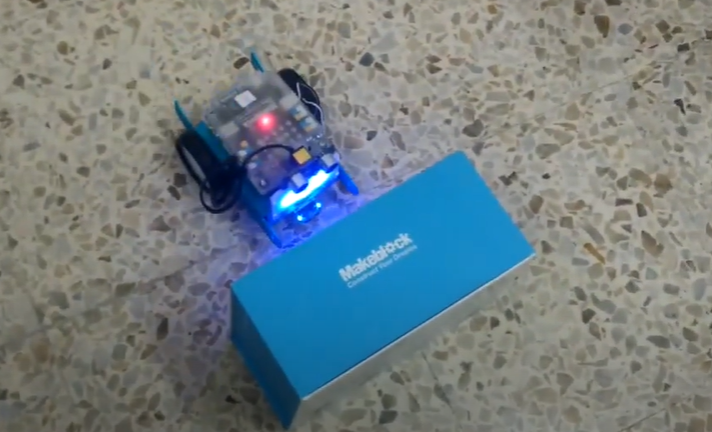
\includegraphics[width=0.5\textwidth]{muro1.png}	
			\label{img:muro1}
		}
	\end{subfigure}
	\begin{subfigure}
		[Otro ejemplo de solución para el ejercicio de no chocar]{
			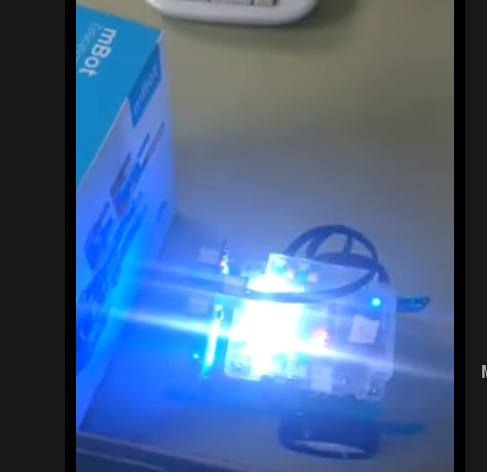
\includegraphics[width=0.5\textwidth]{muro2.png}	
			\label{img:muro2}
		}
	\end{subfigure}
	
	\caption{Ejercicio de no chocar realizado en clase}
	\label{img:muroEjercicio}
\end{figure}

\textbf{Ejercicio extra}. Siempre podemos refinar algo más el ejercicio para que, además de pitar, el robot vaya disminuyendo la velocidad según se acerque al muro hasta, finalmente, pararse. Esto sería una aproximación un poco más cercana al aparcamiento autónomo que llevan incorporado algunos de los coches más modernos.\\
Como ampliación, este ejercicio puede adaptarse para meter la funcionalidad secundaria dentro de \textit{funciones} (en Scratch, nuevo bloque), con un parámetro de entrada del que dependerá la velocidad o la frecuencia de pitido. Estas funciones serán llamadas más tarde, desde el programa principal, con el parámetro de entrada correspondiente a cuánto de cerca esté el robot de la pared. Obviamente, esta funcionalidad no la podremos introducir nada más empezar con los sensores. La experiencia nos demuestra que es mejor esperar a que sean los propios alumnos los que creen las necesidades, y la necesidad de una \textit{función} no la verán hasta que no tengan programas muy grandes (con muchos bloques) y difíciles de leer; será entonces cuando ellos mismos pidan de forma natural paquetizar el código.\\
Esta ampliación la reservaremos, por tanto, para retormarla cuando hayamos visto otro ejercicio en el que sí se necesiten las funciones. Como los alumnos guardan los escenarios con el código de los ejercicios, será fácil retormarlo para cambiarlo.

\item[Luces automáticas]\label{ej:lucesAuto}
En este ejercicio utilizaremos el sensor de luz, también integrado en la placa. Siguiendo la idea de `programar comportamientos de la vida diaria', en este caso desarrollaremos el sistema de las luces de un coche. Éstas se encienden automáticamente cuando no hay luz, bien porque fuera de noche, bien porque fuera un día nublado. Es decir, que si sólo programáramos las luces para que se encendieran a partir de las 8 de la noche, porque es la hora a la que en verano debiéramos encender las luces, en invierno estaremos horas sin luz pues anochece mucho antes. Por tanto, necesitaremos un sistema que nos valga siempre, no dependiendo de la hora a la que anochezca o de si el día es nublado o despejado. \\
Este ejercicio es muy simple por naturaleza, así que lo utilizaremos para introducir un método de cálculo del valor de referencia de la luz ambiental:
al principio del ejercicio, hemos comprobado el nivel de luz ``a mano''. Si cambiamos el sitio, o cualquier otro factor, habrá que volver a sacar este nivel barrera. Para tener que evitar hacer esto, metemos la comprobación en el programa principal, al principio del código. \\
El nivel de luz ambiente que se usará como nivel umbral se obtiene leyendo el nivel de luz del sensor durante \textit{n} veces (10, por ejemplo), sumándolos y dividiéndolos entre \textit{n}; es decir, se hace una media aritmética básica de todos los niveles de luz que se hayan leído. En Scratch se meterá en un bucle el lector del sensor, combinándolo con esperas para coger valores diferentes, y se irá sumando en una variable (a sí misma); después se dividirá ente el número de veces que se hayan dado vueltas al bucle. 

\begin{figure}[h]
	\centering
	\includegraphics[scale=1.2]{variableluz.png}	
	\caption{Variables en Scratch}
	\label{img:variableluz}
\end{figure}


A partir de calcular este valor umbral, se programará el robot para que, si apagamos las luces, se enciendan los LED de la placa (que sería el equivalente a las luces del coche).\\
Esta ampliación del ejercicio nos sirve para explicar el modo correcto de establecer `condiciones de entorno'. Es decir, el entorno tiene unas características, que casi nunca serán fijas o deterministas y que se necesitan como datos para un desarrollo más sólido frente a errores o cambios en el entorno. Además, también servirá para aprender el concepto de \textit{variable} de programación. Una variable es una ``caja'' donde se guarda un valor que vamos a querer utilizar más tarde. En este caso, el valor de la suma de las lecturas consecutivas del lector. Una posible solución al ejercicio se muestra en la imagen \ref{img:lucesautomaticas} \\
Este método de establecer el entorno en variables que se vayan a utilizar y, sobre todo, la necesidad de ello, se volverá a trabajar, con el ánimo de consolidar lo aprendido, en el siguiente ejercicio. 
\begin{figure}[h]
	\centering
	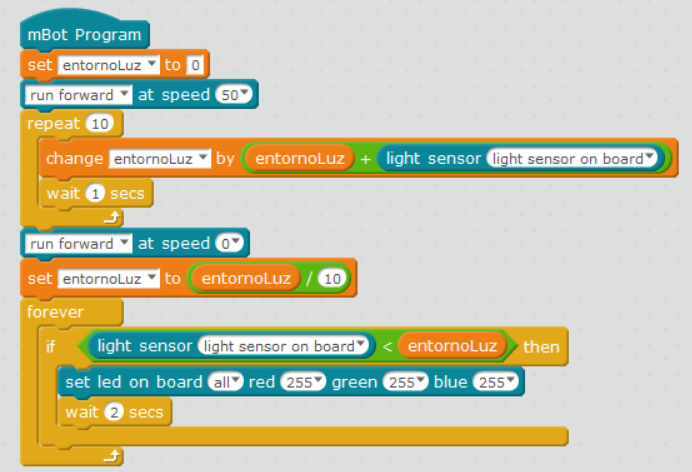
\includegraphics[scale=1]{lucesautomaticas.png}	
	\caption{Ejemplo de solución para las luces automáticas}
	\label{img:lucesautomaticas}
\end{figure}

\item[Huye-luz]\label{ej:huyeLuz}
Esta vez, y no como ejercicio extra sino como uno distinto, diseñamos otro problema con el mismo sensor que ya hemos utilizado en el anterior. El motivo de que sea un ejercicio diferente es que no es un añadido al ejercicio, sino que cambia el requerimiento inicial del problema; éste será que el robot huya de la luz, persiguiéndolo con una linterna.\\
Utilizaremos el mismo método de sacar el valor umbral de referencia pero, esta vez, si estamos por encima de ese valor (en vez de por debajo como antes), el robot tendrá que huir, dando marcha atrás y girando. Una posible solución al ejercicio trabajado en clase se muestra en la imagen \ref{img:huyeluz}.\\

\begin{figure}[h]
	\centering
	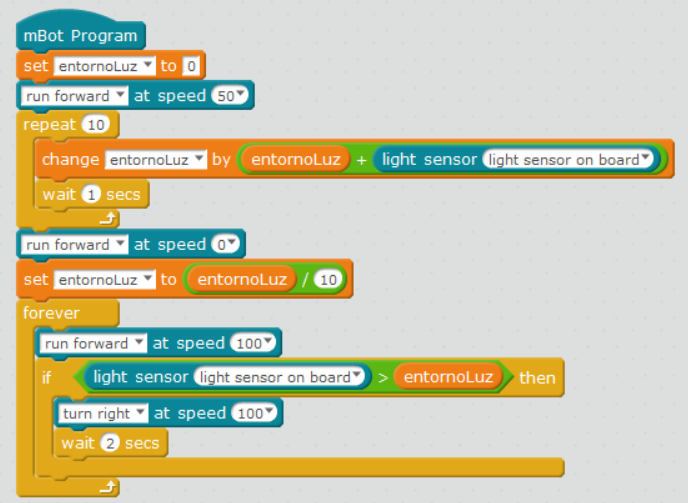
\includegraphics[scale=1]{huyeluz.png}	
	\caption{Ejemplo de solución para el ejercicio Huye Luz}
	\label{img:huyeluz}
\end{figure}

\item[Sigue-líneas]\label{ej:sigueLineas}
El siguiente sensor del robot es el sensor infrarrojo.
Utilizaremos, al principio, el circuito para seguir las líneas que viene en el kit del mBot, que hace un ocho con líneas negras sobre blanco. Es importante que cualquier otro circuito que vayamos a hacer seguir al robot tenga claramente diferenciados el negro y blanco, pues el sensor es binario: está ``tapado'' o no, y si el suelo es oscuro entenderá que es una línea, y se comportará de forma errónea.\\
El objetivo del ejercicio es que el robot siga sin ninguna interacción humana el circuito sin salirse de las curvas. Para los alumnos más jóvenes, atacar este problema directamente resulta demasiado grande y no sabrán como empezarlo sin una guía para aprender a usar el sensor. Lo más difícil de este sensor, en comparación con los otros, es el concepto de \textit{respuesta binaria}. El bloque de Scratch permite acceder a este sensor y darle dos opciones: sensor en negro o sensor en blanco. El primer ejercicio sería, entonces, saber qué significa que el sensor responda negro o blanco (por ejemplo, que encienda las luces), tapándolo y destapándolo, lo que será equivalente a que esté sobre la línea negra o no.\\
La siguiente dificultad es pensar en las diferentes combinaciones de sensor derecho e izquierdo con el blanco y negro. En programación clásica, las combinaciones serías 00, 01, 10, 11, pero esto no vale en Scratch ni para los alumnos. Tendrán que decidir, con el robot y el circuito delante, qué significa cada posibilidad:
\begin{itemize}
	\item El sensor derecho sea negro y el izquierdo negro: está encima de la línea.
	\item El sensor izquierdo sea negro y el derecho blanco: se ha desviado hacia la derecha (o está en una curva a izquierdas).
	\item El sensor derecho es negro y el izquierdo blanco: se ha desviado hacia la izquierda (o está en una curva a derechas).
	\item Los dos sensores leen blanco: se ha salido completamente de la línea.
\end{itemize}
A partir de separar y entender las posibilidades que tenemos con los sensores, el siguiente paso es decidir qué hacer en cada caso de los especificados; se hará programando cada posibilidad a la vez que se diseña la solución.
\begin{itemize}
	\item Si los dos sensores son negros y el robot está en la línea, deberá continuar avanzando sin cambios.
	\item Si el sensor izquierdo es negro pero el derecho no, y el robot está desviado a la derecha, o en una curva, tendrá que girar hacia la izquierda; es decir: seguirá la trayectoria de la curva.
	\item Del revés, si el robot está en una curva desviándose a la izquierda, tendrá que girar a la derecha para seguir la curva.
	\item Si el robot lee los dos sensores en blanco, es que se ha salido del circuito y tendrá que volver a él (girando o dando marcha atrás hasta que el sensor vuelva a ser negro).
\end{itemize}
Una vez solucionado el ejercicio, sólo quedará perfeccionarlo haciendo los giros más precisos para que el movimiento sea más fluido y continuo. La primera vuelta de este perfeccionamiento se hará ajustando las velocidades y las esperas. La segunda vuelta, la forma más correcta de hacerlo, será siguiendo la idea de ``girar hasta estar en el sitio correcto''; es decir, que mantendremos el movimiento deseado (el correspondiente a cada caso), hasta que los dos sensores lean negro y esté otra vez sobre la línea.\\
Como puede observarse, este ejercicio es un ejemplo perfecto de iteraciones Agile.
En la imagen \ref{img:mBotSigueLineas} tenemos la aplicación del ejercicio en clase, que se puede ver completo en vídeo\footnote{\href{https://www.youtube.com/watch?v=Bvspt7w086E}{https://www.youtube.com/watch?v=Bvspt7w086E}}.
\begin{figure}[H]
	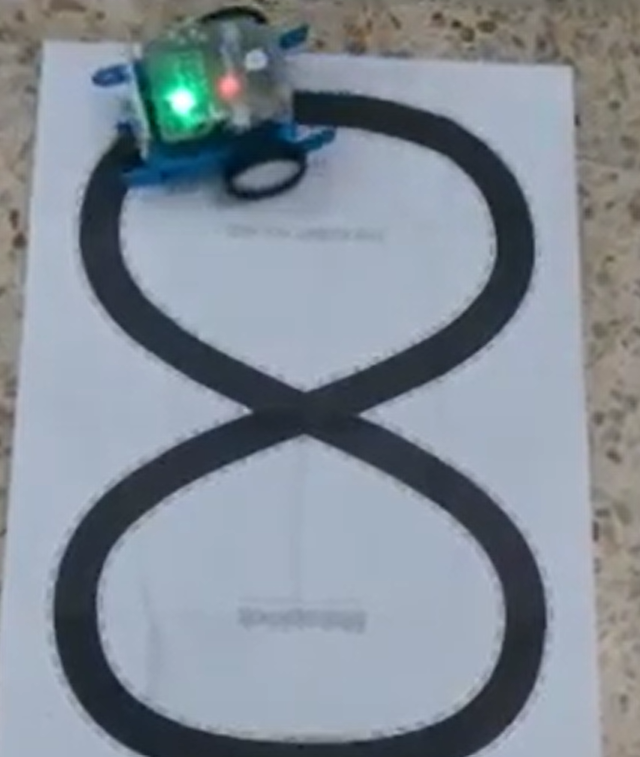
\includegraphics[width=6cm]{mBotSigueLineas.jpg}
	\centering	
	\caption{Ejercicio de Sigue Líneas}
	\label{img:mBotSigueLineas}
\end{figure}

\textbf{Ejercicio extra}. Esta vez no aumentaremos la dificultad ni cambiaremos o ampliaremos las especificaciones del problema, sino que sólo lo pondremos a prueba con diferentes circuitos hechos por los alumnos, cada vez más difíciles o con más curvas, con el fin de demostrar que con una única solución tenemos cubiertos todos los escenarios en todas las situaciones que planteemos. \\
Además, sirve para jugar con el programa que los alumnos han desarrollado, haciéndoles ver que sirve para algo más que sólo `hacerlo'; es importante inculcarles la idea de que programar es divertido y de que ver los resultados es gratificante.

\item[Choca-gira]\label{ej:chocaGira}
Usaremos el mismo sensor de ultrasonido que en el ejercicio del muro (\ref{ej:muro}) pero complicando el requerimiento principal. Esta vez, en lugar de sólo tener que parar para no chocar, el robot intentará evitar el obstáculo para huir de él. El ejercicio básico consistirá en perseguir al robot, poniéndole delante algo con que, de no esquivarlo, chocaría. Para esquivarlo, no sólo tendrá que parar si `lee' un obstáculo delante sino que, deberá girar o dar marcha atrás o las dos cosas: serán los alumnos los que diseñen su propio algoritmo de \textit{esquivado}; no hay una solución única y deberán demostrar su capacidad de decisión delante de una solución abierta. \\
\textbf{Ejercicio extra}. Con el mismo sensor y la misma filosofía que anteriormente, esta vez diseñaremos un algoritmo para \textit{atravesar} los obstáculos y poder continuar la carrera, no para evitarlos y huir de ellos. \\
El propósito es reforzar la autonomía de los alumnos a la hora de buscar una solución, no sólo de implementar un algoritmo (una solución) dado. La diferencia con la carrera de obstáculos del primer apartado de este mismo capítulo, en \ref{ej:carreras}, es que la disposición de estos obstáculos no será fija, sino que el robot deberá ser capaz de solucionar cualquier circuito.
\end{description}

\subsection{Prácticas con aplicaciones}\label{subsec:practicasaplicaciones}
En las dos secciones previas se ha explicado cómo utilizar los sensores y actuadores propios del mBot con el lenguaje de programación Scratch, y se han propuesto ejercicios para practicar todos ellos. Sin embargo, y aunque siempre se ha intentado hacer estos ejercicios lo más reales posibles, a la hora de ponerlo en práctica podemos ver que los alumnos los superan fácilmente y que, en cuanto tienen resuelto el algoritmo, piden opciones que hacerle o le buscan formas distintas con las que poder jugar con el robot. \\
Con ese propósito, para la última parte del curso de Scratch, y ya teniendo en cuenta las herramientas de programación trabajadas hasta ahora, en esta sección propondremos algunos ejercicios más completos y que requerirán de varios sensores y actuadores conjuntos, con comportamientos más complejos y con un propósito más específico. Seguiremos trabajando la programación, reforzando los conceptos de \textit{funciones, variables, orden secuencial, ejecuciones bloqueantes, bucles anidados a condiciones, etc}. \\
Otro propósito de esta sección es el aprendizaje y autonomía de los alumnos a la hora de solucionar un problema. Es decir, no ya de dar la solución programada a un algoritmo, sino de diseñar ellos mismos ese algoritmo que compone la solución. A base de intentos, y distintas iteraciones, el refinamiento de la solución será un punto importante. Seguiremos la idea de la metodología \textit{Agile}: diseño, desarrollo, prueba, rediseño. A pesar de haber seguido este método durante todo el curso, ahora es cuando mejor se puede poner en práctica debido a la naturaleza más continua de los ejercicios (no durarán sólo un día o una iteración).

\begin{description}
	\item[Lucha de Sumo]\label{ej:sumo}
	Con este primer proyecto se pretende demostrar a los alumnos que son capaces de programar comportamientos que pueden usarse de forma completa y única, sin ser necesariamente sólo una pequeña parte de un comportamiento más completo. Es decir, en el caso de las luces automáticas o del sistema de detección de muros, los programas formaban parte de un comportamiento completo al que podríamos referirnos como \break `comportamiento robótico de un coche'; no tenían una aplicación directa por ellos solos. Sin embargo, en este ejercicio que nos ocupa, el comportamiento se programará desde el principio y al completo, con el fin de que los alumnos puedan ver y jugar con un programa hecho por ellos de forma íntegra. \\
	El objetivo del juego es simular un combate de sumo en el que los robot serían los luchadores. Se juega dentro de un ring, si un robot se sale, pierde; un robot, para ganar, deberá sacar al otro del ring. \\
	Para perseguir al otro ``luchador'', utilizaremos el lector de distancia. Si no tenemos nada a \textit{x} distancia, haremos girar al robot y avanzar un poco, así hasta que (y el bloque de control es este `hasta que') tengamos un obstáculo a menos de esa distancia \textit{x}, momento en el cual pararemos de girar e iremos en la dirección en la que está el obstáculo (el otro robot). Como el objetivo es sacar al otro robot del ring, pero no salir de él, si captáramos con el sensor de Sigue Líneas que una o las dos líneas están tapadas (en negro), mandaremos al robot parar. Si las dos líneas estuvieran en negro, y hubiera un obstáculo (un robot) muy cerca, significaría que hemos ganado. Si no, que tenemos que seguir buscando al contrincante.\\	
	Como se puede observar, en este ejercicio se tendrán que mantener muchos sensores y posibles variaciones a la vez, por lo que los alumnos deberán tener muy en cuenta todas las variantes y la posibilidad de que una combinación niegue a la otra. Por ejemplo, que el robot no se salga del campo es prioritario, así que esa condición deberán considerarla la primera, antes de considerar si tienen delante el otro robot. Es decir, esa condición es bloqueante para considerar el resto.\\
	Como todas esas condiciones serán bloques de condición anidados, el código enseguida se haría ilegible, por lo que ahora más que nunca, es imprescindible utilizar funciones. Cada función será un comportamiento predefinido y que siempre será igual. Estas funciones serían las siguientes:
	\begin{itemize}
		\item No salirse del campo. El robot siempre hará lo mismo cuando se encuentre una de las líneas que delimitan el campo. Tendrá las dos opciones, que tenga un obstáculo delante, o que no. Con cada una de estas opciones, tendrá un comportamiento.
		\item Correr hacia el adversario. En cuanto el robot detecte, a una distancia predefinida, que el contrincante está delante suya, correrá más rápido, y siempre a la misma velocidad. 		
	\end{itemize} 
	Además, todos esos valores \textit{constantes}, como las distintas velocidades o la distancia a la que considerar que el robot contrario está cerca, siempre serán \textit{variables globales}, en vez de valores numéricos embebidos en el código.
	
	\item[Laberinto] \label{ej:laberinto}
	Siguiendo la misma línea de `proyecto', y de integración de conocimientos, esta vez proponemos el diseño de resolución autónoma de un laberinto. \\
	Lo primero que debemos comentar es el algoritmo de resolución del laberinto, teórico, que implementaremos en código. Dado que la intención es la ``robotización'' del proceso, haciéndolo independiente de la acción humana, nos basaremos en una de las formas clásicas de resolución de laberintos: siempre seguir la pared que se tenga a la derecha (o a la izquierda, pero siempre el mismo lado). Es decir, para salir de un laberinto, deberemos seguir desde la entrada del mismo, la pared que tengamos a la derecha; en caso de encontrar un giro (una esquina) deberemos seguirla también. Este método se conoce como `método de la mano derecha' y sirve para la mayoría de laberintos. En la siguiente imagen se observa con claridad:
	\begin{figure}[H]
		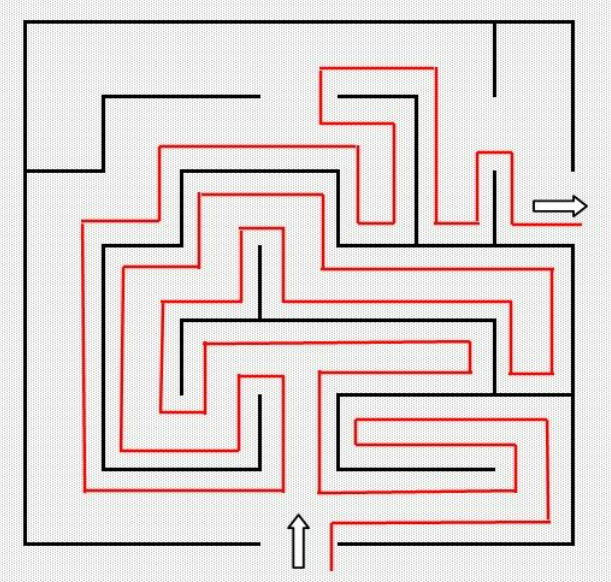
\includegraphics[scale=0.5]{laberinto.png}
		\centering
		\label{img:laberinto}
		\caption{Método de la mano derecha}
	\end{figure}
	Este método no asegura el camino más corto sino la certeza de la resolución. De hecho, en la imagen puede observarse que si hubiéramos utilizado el método de la mano \textit{izquierda}, el camino habría sido más corto. Sin embargo, como el objetivo es utilizar un sólo método para todos los posibles laberintos, escogeremos uno e implementaremos todos los alumnos el mismo. \\
	Lo primero sería la preparación, del robot y del entorno. Como necesitaremos que el robot vea paredes a los lados, y no solo de frente, utilizaremos el sensor Sigue Líneas como `lector de paredes'; adaptaremos al robot cambiando de lugar este sensor:
	\begin{figure}[H]
		\includegraphics[width=6cm]{mBotlaberinto.jpg}
		\centering
		\label{img:mBotlaberinto}
		\caption{Preparación del mBot con el sensor sigue líneas lateral}
	\end{figure}
	Esta necesidad de `cambiar' al robot serán los propios estudiantes quiénes la verán, durante el proceso de toma de requerimientos, y después de haber conocido el algoritmo de la mano derecha. Para este proceso de preparación, será necesario haber montado un laberinto de pruebas, por ejemplo de porexpan (cualquier laberinto simple, el de la imagen por ejemplo). Verán la necesidad de conocer si hay una pared al lado o no, y si hay otra enfrente o no, cuando físicamente vean el robot dentro del laberinto e intenten resolver el algoritmo. \\
	Siguiendo el mismo procedimiento Agile que durante el curso, programaremos el \break comportamiento en etapas unitarias, en modo \textit{bottom-up}, y con su fase de test entre cada una (varias fases de test, de recalibración de velocidades, de perfeccionamiento, etc):
	\begin{enumerate}
		\item Idea principal del algoritmo: seguir la pared de la derecha. Para ello utilizaremos el sensor infrarrojo Sigue Líneas de forma que, si están los dos sensores tapados (negro) hay pared y debemos seguir avanzando; si están los dos sensores destapados (blanco) hemos pasado una esquina ``a derechas'' (sin tener pared delante) y tenemos que girar a la derecha \textit{hasta que} los dos sensores vuelvas a estar tapados.
		\item Esta condición anterior es así \textit{mientras que} el sensor de distancia delantero no tenga una pared a \textit{x} distancia. Si están los dos sensores infrarrojos tapados, pero tenemos una pared delante, significará que tenemos una esquina ``a izquierdas'' y deberemos girar hacia la izquierda \textit{hasta que} no haya pared delante.
		
	\end{enumerate}
	El trabajo más importante para el estudiante será el diseño de estados' del robot; qué estados son bloqueantes (van antes en el código) y el orden en que analizar todas las variables disponibles.
	
	\begin{figure}[H]
		\includegraphics[scale=0.7]{laberintoSolucion.png}
		\centering
		\label{img:laberintoSolucion}
		\caption{Ejemplo de solución en clase para el laberinto}
	\end{figure}
	
	\item [Aparcamiento Autónomo] \label{ej:aparcamiento}
	Este ejercicio es posible con la misma configuración de sensores que la del laberinto. El propósito es programar el comportamiento de un sistema de aparcamiento de un vehículo moderno, que cuando encuentra un hueco suficientemente grande, aparca de forma autónoma. Las distintas fases de diseño, serían las siguientes:
	\begin{enumerate}
		\item El primer problema que atajar es qué significará para el robot un sitio ``suficientemente grande''. La premisa del entorno será una `pared' creada con porexpan, o algo equivalente, que en un momento determinado desaparece porque hay un hueco para aparcar. Por tanto, utilizaremos el sensor lateral de forma parecida al ejercicio anterior: mientras que los dos sensores estén en negro, tendremos que seguir avanzando.
		\item Cuando los dos sensores laterales estén en blanco, significará que hemos encontrado un \textit{posible} hueco. Si es suficiente o no, como el robot no tiene capacidad de calcular su propio tamaño, vendrá determinado por cuánto tiempo avancemos (iniciando una variable tiempo a 0) \textit{hasta que} los dos sensores vuelvan a estar tapados. El tiempo que tarde en encontrar un hueco suficientemente grande lo calcularemos una vez, y lo utilizaremos como valor referencia en el programa principal: si es mayor que \textit{T}, será suficiente, si no, hay que seguir buscando.
		\item Tras encontrar un hueco, el robot deberá parar y dar marcha atrás (girando ligeramente) \textit{hasta que} el sensor delantero tenga un valor de referencia, lo que significará que tiene un 'coche' delante. 
		\item Este proceso puede perfeccionarse todo lo que los estudiantes quieran, para mejorar el aparcamiento y que sea más preciso.		
	\end{enumerate}
	Una variación interesante de este ejercicio, una vez que los estudiantes hayan programado el algoritmo, es cambiar la disposición de los sensores: poner en el lateral el sensor de distancia de ultrasonidos, y delante el infrarrojo. El procedimiento es el mismo, pero deberán ajustar los valores, re-calcular las constantes de referencia y re-diseñar los detalles de implementación. Lo más importante es que aprenden que las soluciones a un mismo problema no son únicas.
	\begin{figure}[H]
		\includegraphics[width=6cm]{mBotaparcamiento.jpg}
		\centering
		\label{img:mBotaparcamiento}
		\caption{Ejercicio de aparcamiento autónomo}
	\end{figure}
	Otra posible variación, útil en caso de que haya alumnos que trabajen a diferentes velocidades (algo muy habitual) es añadirle la funcionalidad trabajada en otros ejercicios, por ejemplo que emitiera sonido con la marcha atrás.
\end{description}


\section{Programación robótica con Python}\label{sec:Python}
Esta segunda parte del curso educativo está supeditada a que los alumnos hayan tenido una buena acogida de los contenidos de la primera etapa, tanto educativa como temporalmente. Si no fuera así, y el curso de Scratch durará todo el curso natural, la parte de Python se planteará como un segundo curso. Es importante que hayan aprendido globalmente conceptos de programación para poder introducir el concepto de `código', con todas las normas que ello conlleva. Scratch para ello es una ventaja frente a otros lenguajes ``infantiles'', pues es una suerte de \textit{pseudocódigo}, frente a otros que no contienen nada de texto y son completamente pictográficos (orientados a alumnos aún más jóvenes, que no han empezado o terminado de aprender a leer). \\
Se han diseñado una serie de ejercicios de dificultad progresiva, para introducir a los estudiantes en la programación clásica con el lenguaje de texto Python y dar un paso más en su aprendizaje en robótica, utilizando la plataforma diseñada en este Trabajo Fin de Grado PyBoKids-2.0.
\subsection{PyBoKids 2.0}
El objetivo de la plataforma desarrollada es ofrecer un medio para que personas que no han utilizado nunca un lenguaje formal de programación, programen el robot mBot con ese lenguaje. El hecho en sí es complicado, ya que tiene varios hándicaps que superar: la edad de los alumnos, la complicación de empezar a programar y además, de aprender un lenguaje de cero, sumada al hecho de estar utilizándolo para robótica, y no sólo programación ``básica''. Esta plataforma ofrece una posibilidad para no depender del lenguaje de la placa, Arduino, más complejo y menos manejable . \\
El uso en clase de  PyBoKids-2.0 será muy sencillo:
\begin{enumerate}
	\item Los robot llevarán ya grabado el programa residente de Arduino, para que no sea necesario hacerlo en clase. Sin embargo, si un alumno u alumna quisiera hacerlo de forma independiente, el procedimiento de instalación está explicado en \ref{list:InstalacionArduino}. Será necesario: 
	\begin{itemize}
		\item Instalación del Arduino IDE
		\item Descargar las librerías de Arduino y el programa residente del repositorio de PyBoKids-2.0\footnote{\href{https://github.com/JdeRobot/PyBoKids}{https://github.com/JdeRobot/PyBoKids}}
		\item Incluir las librerías según las instrucciones del Capítulo \ref{cap:infra} comentadas
		\item Abrir el fichero de extensión .ino del programa residente anteriormente descargado, y grabarlo en la placa
	\end{itemize}
	\item Descargar e instalar Python 3.0 según las instrucciones en \ref{list:instalacionPython}
	\item Descargar la biblioteca de PyBoKids (fichero \textit{Library\_mbot\_v1}) y el fichero \textit{esqueleto.py} desde el repositorio de PyBoKids-2.0, y guardarla localmente en el directorio donde vayamos a trabajar.	
	\item Abrir el fichero \textit{esqueleto} y guardarlo con el nombre del programa que vayamos a realizar, para guardar una copia (y no sobreescribirlo).
\end{enumerate}

Como puede verse, el proceso es muy sencillo, y al alcance de los alumnos. 
\subsection{Prácticas de lenguaje}
Como sería la primera vez que utilizan un lenguaje de programación textual clásico, es necesario introducirlos en las normas, en la sintaxis básica y en la forma de ejecución. Para ellos hemos preparado unos ejercicios simples sólo de lenguaje, a los que dedicar poco tiempo (pues no son de robótica), a modo de introducción.
\begin{description}
\item [Hola mundo] Como en cualquier curso introductorio de lenguaje, el primer 'Hola mundo' es fundamental para enseñar a los alumnos a abrir un fichero nuevo, guardarlo, y ejecutarlo. En este caso, usaremos el IDE nativo de Python en Windows, al igual que su shell. Es por tanto, muy fácil ejecutar un programa guardado con la opción propia del IDE.
	\begin{figure}[H]
		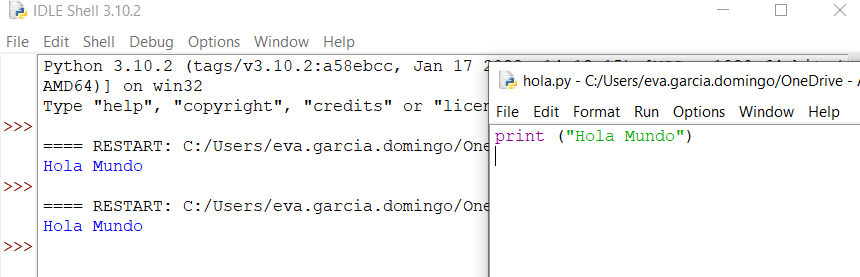
\includegraphics[scale=0.6]{hola.png}
		\centering
		\label{img:holamundo}
		\caption{Hola Mundo en Python}
	\end{figure}
\item [Calculadora] Para aprender cómo usar variables en Python, y cómo acceder a ellas, haremos algo tan simple como útil: guardar dos valores diferentes en dos variables, \textit{a} y \textit{b}, e imprimir por pantalla la suma, resta, multiplicación y división de ellas. 
\item[Calculadora II] El mismo ejercicio anterior, pero pidiendo los valores de \textit{a,b} por teclado. 
\item[Cumpleaños feliz] El objetivo de este ejercicio es que aprendan que hay diferentes tipos de objeto (no es el mismo tipo de objeto los números de la calculadora, que un \textit{String} de texto) que se pueden almacenar en una variable, y que aprendan a usar un bucle \textit{for..i in range()}, con el objetivo de no tener que repetir varias líneas de código cada vez que la canción repite el mismo texto. Además, el número de veces que vayamos a repetir la canción será un valor pedido por teclado.
\item [Suma progresiva] Para trabajar los bucles \textit{while}, haremos una suma aritmética utilizando un valor que iremos incrementando en cada pasada del bucle (\textit{i}). Primero haremos 5 iteraciones, después 10, etc, para que los alumnos vean cómo cambiar fácilmente el código para obtener el resultado deseado. También será importante que aprendan la diferencia entre \textit{menor que} y \textit{menor o igual que}, ya que el bucle hará una interación más o menos.
\begin{lstlisting}[language=python]
i = 0
while i < 6:
 print(i+1)
 i += 1
\end{lstlisting}
\item [Calculadora III] Para utilizar los condicionales, haremos una pregunta tan simple como \textit{¿y si intentamos dividir por cero?} que tendrán que resolver. Además, al tratar de dividir por cero, comprobarán cómo son los errores en Python (los errores son algo que deben aprender a leer y manejar).
\begin{figure}[H]
	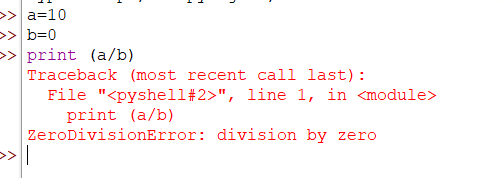
\includegraphics[scale=1.4]{errorPython.png}
	\centering
	\label{img:error}
	\caption{Error en Python}
\end{figure}
\end{description}

Habiendo utilizado variables, bucles y condiciones, se puede empezar a programar el mBot de forma progresiva, pues el objetivo es que re-aprendan todos estos conceptos con una programación formal usando un lenguaje textual.
\subsection{Prácticas robóticas}
Como se mencionó brevemente en el final del Capítulo \ref{cap:PyBoKids}, para esta etapa del curso educativo, se ha preparado un esqueleto de programación en Python, con el objetivo tanto de facilitar la programación a los estudiantes, como de guiarles en unas buenas prácticas (entre ellas, la obligatoriedad de la indentación propia de Python). Este esqueleto contiene la importación del módulo de la biblioteca, y una guía de dónde corresponde cada parte del programa. Lo utilizaremos, al menos las primeras veces, para hacer los ejercicios diseñados. Más adelante, y dependiendo del ejercicio, harán cambios en él, es sólo una guía para empezar. Además, en la biblioteca, tenemos una ayuda programada para mostrarle al alumno las posibles funciones que tiene disponibles (la función, al no ser una ayuda de Python ``al uso'', se llama \textit{functions\_mbot} y está pre-programada en el esqueleto):

\begin{lstlisting}[language=python,caption={Esqueleto proporcionado a modo de ejemplo}]
# -- Esto es un comentario

# -- Aqui los modulos necesarios
import sys
import serial
from time import sleep
from Library_Mbot_v1 import *


#-- Poner aqui las variables globales, si se necesitan

#-- Sacar mensaje inicial: que va a hacer el robot

try:
#--Escribe aqui el programa principal
	functions_mbot()
except KeyboardInterrupt:
	send_Quit(serial)

sys.exit(0))
\end{lstlisting}
\begin{figure}[H]
	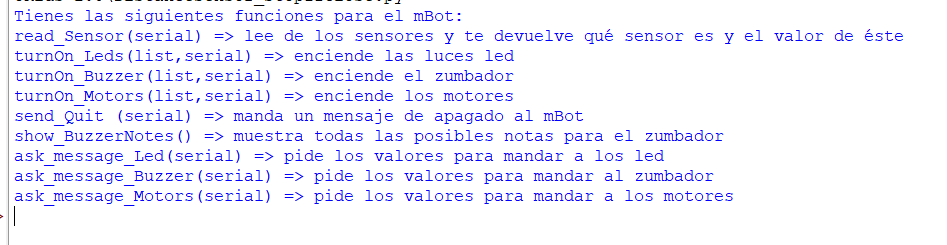
\includegraphics[scale=0.6]{ayuda.png}
	\centering
	\label{img:ayuda}
	\caption{Ayuda sobre el mBot}
\end{figure}

A continuación explicaremos los ejercicios programados para esta parte del curso. Muchos de ellos, al ser los mismos que en Scratch en la sección \ref{sec:scratch} no los repetiremos a no ser que sean necesarias aclaraciones o ayudas debido al cambio de plataforma.\\

Aunque no vaya a hacer ningún efecto, lo primero que deben aprender es la forma de conectarse al robot. Se les explicará haciendo referencia a la conexión en Scratch, que también era necesaria, y se les mostrará cómo usar la función preparada para ello 
\begin{lstlisting}[language=Python]
	serial = open_PortSerial('com3')
\end{lstlisting}
Este primer ``programa'' no ejecutará nada, sino que la forma de ver que ha funcionado correctamente es comprobar que no genera fallo. Si cambiáramos el puerto en la función, podríamos comprobar que no funciona.
\begin{description}
	\item [Luces LED] Al ser el actuador más sencillo, será el primero que utilicemos. Lo primero es la toma de decisiones (qué queremos que el robot haga), después debemos pasar esos datos a lenguaje, y después utilizar la biblioteca del mBot. Es importante explicarles cómo funcionan las funciones de envío de datos. En este caso, cómo hacer un array (una lista) con los datos que queremos empaquetar para enviar al robot.
\begin{lstlisting}[language=python,caption={Solución de referencia del ejercicio de las luces LED para Python}]
# -- Esto es un comentario		
# -- Aqui los modulos necesarios
import sys
import serial
from time import sleep
from Library_Mbot_v1 import *
#-- Poner aqui las variables globales, si se necesitan
serial = open_PortSerial('com3')
#-- Sacar mensaje inicial: que va a hacer el robot
print ("Prueba de led")
try:
	#--Escribe aqui el programa principal
	turnOn_Leds([0,255,0,0],serial)
	sleep(3)
	send_Quit(serial)
except KeyboardInterrupt:
	send_Quit(serial)

serial.close()
sys.exit(0)
\end{lstlisting}
	\item [Carreras] Realizaremos el mismo ejercicio que con Scratch, esta vez enviando los datos a los motores con la biblioteca de PyBoKids-2.0. La toma de decisiones pasará por decidir la velocidad a la que mandar los motores moverse, y por crear el objeto de lista con los valores que enviar. Es notable que este ejercicio se debe realizar con cuidado, ya que continuamos teniendo el robot conectado por cable al PC.
\begin{lstlisting}[language=python,caption={Solución para el ejercicio de carreras en Python}]
# -- Esto es un comentario		
# -- Aqui los modulos necesarios
import sys
import serial
from time import sleep
from Library_Mbot_v1 import *

#-- Poner aqui las variables globales, si se necesitan
serial = open_PortSerial('com3')
#-- Sacar mensaje inicial: que va a hacer el robot

print ("Usar los motores (M1 y M2) componiendo el 
mensaje completo para mandar exactamente los valores")
	
while True:
	try:
		print ("Send new message or quit?")
		cadena=input()
		if (cadena.lower() == 'quit'):
			send_Quit(serial)
			break
		print ("Enter velocity for left motor (-255,255)")
		izdo=input()
		print ("Enter velocity for rigth motor (-255,255)")
		dcho=input()	
		turnOn_Motors([100,100],serial)
	except KeyboardInterrupt:
		send_Quit(serial)
		break
	
serial.close()
sys.exit(0)
\end{lstlisting}
	\item [SOS] Esta vez, para hacer el mismo ejercicio de SOS que anteriormente, elegiremos la nota a la que emitir y las dos duraciones diferentes por teclado. La propuesta es que se repita el SOS tres veces (o \textit{n} veces) y después termine, usando el mensaje \textit{quit} programado.
\begin{lstlisting}[language=python,caption={Solución en Python para el ejercicio S.O.S.}]
# -- Esto es un comentario		
# -- Aqui los modulos necesarios
import sys
import serial
from time import sleep
from Library_Mbot_v1 import *

#-- Poner aqui las variables globales, si se necesitan
serial = open_PortSerial('com3')
#-- Sacar mensaje inicial: que va a hacer el robot
print ("Mensaje de socorro con el zumbador")

try:
	#--Escribe aqui el programa principal
	Mensaje_Zumbador_punto = ask_Message_Buzzer(serial)
	Mensaje_Zumbador_raya = ask_Message_Buzzer(serial)
	for i in range(6):
		for i in range (3):
			turnOn_Buzzer(Mensaje_Zumbador_punto,serial)
		for i in range (3):
			turnOn_Buzzer(Mensaje_Zumbador_raya,serial)
		for i in range (3):
			turnOn_Buzzer(Mensaje_Zumbador_punto,serial)
		sleep(3)
		send_Quit(serial)
except KeyboardInterrupt:
	send_Quit(serial)

serial.close()
sys.exit(0)
\end{lstlisting}
	\item [Sensores] Para aprender a usar la forma de leer de los sensores de PyBoKids-2.0, les propondremos leer del sensor, comprueben que es el que necesitan (con un bloque \textit{if..else}) e impriman el valor del sensor por pantalla. Además, así aprenden a acceder a un Array, no sólo a crearlo. \\
	Haremos esto con los tres sensores, para aprender cómo usarlos y poder pasar a programar los ejercicios mezclando sensores y actuadores. Lo más importante, obviamente aparte de aprender a usar la plataforma, es que vean la necesidad de un bucle para mantener leyendo del sensor al robot, ya que el valor puede cambiar en cualquier momento.
\begin{lstlisting}[language=python,caption={Solución para distinguir los sensores en Python}]
# -- Esto es un comentario		
# -- Aqui los modulos necesarios
import sys
import serial
from time import sleep
from Library_Mbot_v1 import *

#-- Poner aqui las variables globales, si se necesitan
serial = open_PortSerial('com3')
#-- Sacar mensaje inicial: que va a hacer el robot

print ("Lee de los sensores para distinguir de 
cual viene el mensaje")

while True:
	try:
		#--Escribe aqui el programa principal
		sensorMessage = read_Sensor(serial)
		if (sensorMessage == -1):
			pass
		else:
			if (sensorMessage[0] == 'distance'):
				print ("distance: " + sensorMessage[1])
			elif (sensorMessage[0] == 'siguelineas'):
				print ("siguelineas: " + sensorMessage[1])
			elif (sensorMessage[0] == 'luz'):
				print ("sensor de luz: " + sensorMessage[1])
	except KeyboardInterrupt:
		send_Quit(serial)

serial.close()
sys.exit(0)
\end{lstlisting}

	\item [Luces rojas si hay un muro delante] Una vez comprobados los sensores, el siguiente paso es programar los ejercicios más complicados, que requieren de mayor programación al mezclar la lectura de sensores, el tratamiento de los datos, la decisión sobre ellos y el envío de datos a los actuadores. Aún así, el más sencillo de ellos sigue siendo el módulo \textit{LED}, por lo que empezaremos encendiendo una luz roja si el valor del sensor de Distancia es menor que un valor umbral (guardado como valor global o pedido por pantalla) y verde en caso contrario (es importante recordar que el sensor recoge un valor máximo de 400 cm).
\begin{lstlisting}[language=python,caption={Solución del ejercicio de LEDs y sensor de Distancia en Python}]
# -- Esto es un comentario		
# -- Aqui los modulos necesarios
import sys
import serial
from time import sleep
from Library_Mbot_v1 import *

#-- Poner aqui las variables globales, si se necesitan
serial = open_PortSerial('com3')
#-- Sacar mensaje inicial: que va a hacer el robot
	
print ("Lee del sensor de distancia (ultrasonic) y enciende LED 
rojo si la pared esta muy cerca y verde si no")

while 1:
	try:
		sensorMessage = read_Sensor(serial)    
		if (sensorMessage == -1):
			continue
		else:
			if (sensorMessage[0].lower() == 'distance'):
				if (sensorMessage[1] < 10):
					turnOn_Leds([0,255,0,0],serial)
				else:
					turnOn_Leds([0,0,255,0],serial)
	except KeyboardInterrupt:
		send_Quit(serial)
		break
	
serial.close()
sys.exit(0)
\end{lstlisting}
	\item [Condicionales] Lo más interesante de poder utilizar el PC para la entrada de datos es la diferencia de órdenes que enviar al robot. Así, con el mismo programa podremos utilizar actuadores diferentes dependiente de lo que escribamos por teclado, utilizando comparadores y bloques condicionales para, por ejemplo, encender un LED u otro, el zumbador, o los motores. En este caso pondremos también el foco en la opción por defecto de los bloques condicionales, concepto muy importante en pensamiento computacional y robótica
\begin{lstlisting}[language=python,caption={Solución de referencia del ejercicio sobre condicionales}]
# -- Esto es un comentario		
# -- Aqui los modulos necesarios
import sys
import serial
from time import sleep
from Library_Mbot_v1 import *

#-- Poner aqui las variables globales, si se necesitan
serial = open_PortSerial('com3')
#-- Sacar mensaje inicial: que va a hacer el robot

print ("Opciones diferentes para hacer")

while 1:
try:
	#--Escribe aqui el programa principal
	print ("Escribe lo que quieres hacer: quit,
	 leds, motores, o zumbador")
	cadena=input()
	if (cadena.lower() == 'quit'):
		send_Quit(serial)
		break
	elif (cadena.lower() == 'leds'):
		print ("Color?: rojo, azul, verde")
		cadenacolor=input()
		if (cadenacolor.lower() == 'red'):
			turnOn_Leds([0,255,0,0],serial)
		elif (cadenacolor.lower() == 'verde'):
			turnOn_Leds([0,0,255,0],serial)
		elif (cadenacolor.lower() == 'azul'):
			turnOn_Leds([0,0,0,255],serial)
		else:
			print ("color equivocado")
			continue
	elif (cadena.lower() == 'motores'):
		print ("rapido o lento?")
		cadenavelocidad = input()
		if (cadenavelocidad.lower() == 'rapido'):
			turnOn_Motors([255,255],serial)
		if (cadenavelocidad.lower() == 'lento'):
			turnOn_Motors([100,100],serial)
		else:
			print ("velocidad equivocada")
			continue
	elif (cadena.lower() == 'motores'):
		print ("agudo o grave?")
		cadenanota = input()
		if (cadenanota.lower() == 'agudo'):
			turnOn_Buzzer([659,3],serial)
		elif (cadenanota.lower() == 'grave'):
			turnOn_Buzzer([73,3],serial)
		else:
			print("opcion equivocada")
			continue
	else:
		print("No te he entendido. Escribe exactamente la orden")
		continue

except KeyboardInterrupt:
	send_Quit(serial)

serial.close()
sys.exit(0)
\end{lstlisting}
\end{description}